\begin{frame}{Unitary Evolution \& Measurement}
    \begin{figure}
        \begin{quantikz}
            \lstick{$\ket{0}$} & \gate{H} & \ctrl{1} & \gate{U} & \ctrl{1} & \swap{2} & \ctrl{1} & \qw & \meter{}\\
            \lstick{$\ket{0}$} & \gate{H} & \targ{} & \octrl{-1} & \control{} & \qw & \octrl{1} & \qw & \meter{}\\
            &&&&\lstick{$\ket+$}&\targX{} & \gate{U} & \qw & \meter{}
        \end{quantikz}
        \caption{An Example Quantum Circuit}
    \end{figure}
\end{frame}

\begin{frame}{Unitary Evolution \& Measurement}
    \begin{figure}
            \begin{quantikz}
             
                \lstick{$\ket{0}$} & \gate{H}\gategroup[3,steps=7,style={fill=blue!10, inner xsep=4pt}, background]{{\sc Unitary}} & \ctrl{1} & \gate{U} & \ctrl{1} & \swap{2} & \ctrl{1} & \qw & \meter{} \gategroup[3,steps=1,style={fill=red!10},
                background]{{\sc Measurement}}\\
                \lstick{$\ket{0}$} & \gate{H} & \targ{} & \octrl{-1} & \control{} & \qw & \octrl{1} & \qw & \meter{}\\
                &&&&\lstick{$\ket+$}&\targX{} & \gate{U} & \qw & \meter{}
            \end{quantikz}
        \caption{An Example Quantum Circuit}
    \end{figure}
\end{frame}


\begin{frame}{Unitary Evolution \& Measurement}
    \centering
    \begin{tabular}{p{0.3\linewidth}@{\hspace{0.1\textwidth}} p{0.3\linewidth}}
        \textbf{Unitary Evolution} & \textbf{Measurement} \\[.5em]
        \tabitem Deterministic & \tabitem Probabilistic \\
        \tabitem Reversible & \tabitem Irreversible \\
        \tabitem Intuitive (somewhat)
    \end{tabular}
\end{frame}

\begin{frame}{Measurement-Based Quantum Computer}
    \centering
    \begin{minipage}{0.8\linewidth}
        Two componets:
        \begin{enumerate}
            \item Cluster: Holds the qubits. Substrate for universal computation.
            \item Measurement Device:  Governs the program execution.
        \end{enumerate}
    \end{minipage}
\end{frame}

\begin{frame}{The Cluster: Graph States}
    \centering
    \begin{minipage}{0.3\linewidth}
            \tikz[ baseline={([yshift=-.5ex]current bounding box.center)} ] \graph [
              nodes={draw, circle, inner sep=2.5pt, thick},
              empty nodes,
              edges = {thick}
            ] {
              a -- b -- c;
              d -- e -- f;
              a -- d; b -- e; c -- f;
            };    
    \end{minipage}
    \hspace{0.10\linewidth}
    \begin{minipage}{0.45\linewidth}
        \begin{itemize}
            \item Cluster is a rectengular regular lattice of qubits.
            \item Each qubit is entangled to its neighbouring qubits.
            \item Its quantum state is represented by a graph state.
        \end{itemize}
    \end{minipage}
\end{frame}

\begin{frame}{The Cluster: Graph States}
    \centering
    \begin{minipage}{0.3\linewidth}
        \begin{tikzpicture}[new set=import nodes]
            \begin{scope}[nodes={
              set=import nodes,
              draw, circle,
              fill=red!20
            }]
              \node (k1) at (0, 0) {$\ket{+^{\spaceScript{1}}}$};
              \node (k2) [right=2cm of k1] {$\ket{+^{\spaceScript{2}}}$};
              \node (k3) [below=2cm of k1] {$\ket{+^{\spaceScript{3}}}$};
              \node (k4) [below=2cm of k2] {$\ket{+^{\spaceScript{4}}}$};
            \end{scope}
          
            \graph [
              edges = {line width = 0.2mm}, 
              node distance={15mm},] {
              (import nodes);
              k1 -- ["$CZ_{12}$"] k2 -- ["$CZ_{24}$"] k4;
              k3 -- ["$CZ_{23}$"] k2;
            };
          \end{tikzpicture}
    \end{minipage}
    \hspace{0.10\linewidth}
    \begin{minipage}{0.45\linewidth}
        \begin{itemize}
            \item<1-> A graph has: \begin{enumerate}
                \item A set of vertices \(V = \Set{1, 2, \dots, N}\). Represents qubits
                \item A set of edges connecting some of the vertices \(E \subseteq [V]^2 \;\text{where}\; \abs{E\,} = M\). Represents entanglement patterns.
            \end{enumerate}
            \item<2-> Prepare each qubit in \(\ket+\), apply \(CZ\) if they are entangled.
        \end{itemize}
    \end{minipage}
\end{frame}

\begin{frame}{Measurement Device}   
    \begin{itemize}
    \item Can randomly access the qubits on the cluster
    \item Performs spin measurements on any direction
    \item Recieves measurements patterns as its input.\[\symcal{M} = \Set*{\,\vec{r}_a \given a \in \symcal{C}\,}\]
    \end{itemize} 
\end{frame}

\begin{frame}{Simulating Circuits with MBQC}
        \begin{itemize}
            \item Prove that MBQC is universal
            \item Reuse existing algorithms and code
        \end{itemize}
\end{frame}

\begin{frame}{Simulating Circuits with MBQC}
        \begin{figure}
            \centering
            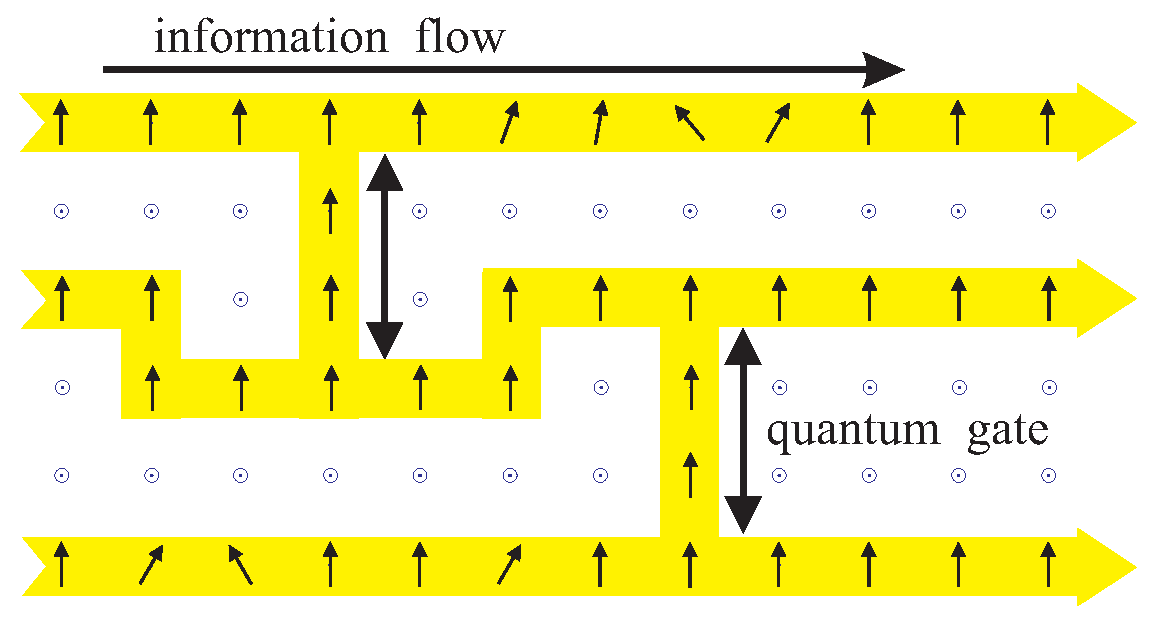
\includegraphics[scale=0.35]{fig/flow.eps}
            \caption{Unitary Gate Simulation Diagram}
        \end{figure}
        \begin{itemize}
            \item Simulate universal gate set \(\cnot=\sigma_x\) and \(R(\alpha, \beta, \gamma)\).
            \item Fix by products after each gate simulation
        \end{itemize}
\end{frame}

\begin{frame}{Simulating Unitary Rotation}
    \centering
    \begin{minipage}{0.3\linewidth}

        \tikz[ baseline={([yshift=-.5ex]current bounding box.center)} ] \graph [
            nodes={draw, circle, inner sep=2.5pt, thick},
            empty nodes,
            edges = {thick}
          ] {
            d[fill=zx_green] -- e[label={$\scriptscriptstyle \alpha$}]  -- f[label={$\scriptscriptstyle \beta$}] -- g[label={$\scriptscriptstyle \gamma$}] -- h;
          };
        
    \end{minipage}
    \hfill
    \begin{minipage}{0.6\linewidth}
        \begin{itemize}
            \item Single qubit measurements on basis \[\symcal{B}(\varphi) = \Set*{\frac{\,\ket0 + e^{i\varphi}\ket1}{2}, \frac{\,\ket0 - e^{i\varphi}\ket1}{2} \,}\] that simulate \[  \sigma_x^s \, H P(\varphi) = \sigma_x^s \, J(\varphi),
            \]
            \item MBQC implements \[
                \underbrace{\sigma_x^{s_2 + s_4} \sigma_z^{s_1 + s_3}}_{U_{\Sigma,R}} \underbrace{J(0) J(\gamma) J(\beta) J(\alpha)}_{R(\alpha, \beta,\gamma)}
              \] through 4 adaptive measurements.
        \end{itemize}
    \end{minipage}
\end{frame}

\begin{frame}{Simulating \(\cnot\)}
    \centering
    \begin{minipage}{0.3\linewidth}
        \tikz[ baseline={([yshift=-.5ex]current bounding box.center)} ]
        \graph [
          nodes={draw, circle, inner sep=2.5pt, thick},
          empty nodes,
          edges = {thick}
        ] {
          d[fill=zx_red, label=left:{Input}] -- e[fill=zx_red] -- f[label=right:{Output}];
          a[draw=none] --[draw=none]  g[label=right:{Control}] -- e;
        };      
    \end{minipage}
    \hfill
    \begin{minipage}{0.6\linewidth}
        \begin{itemize}
            \item Apply \(\sigma_x\) measurements on red vertices.
            \item MBQC implements \[
                U_{\cnot}' = U_{\Sigma, \cnot} U_{\cnot}
            \] with a by-product \[
                U_{\Sigma, \cnot} = \left(\sigma_x^{\scriptscriptstyle(3)}\right)^{s_2} \left(\sigma_z^{\scriptscriptstyle(3)}\right)^{s_1}\left(\sigma_z^{\scriptscriptstyle(4)}\right)^{s_1}
              \] through 4 adaptive measurements.
        \end{itemize}
    \end{minipage}
\end{frame}

\begin{frame}{Additional Patterns}
    \centering
    \begin{itemize}
        \item Measuring a wire of qubits on \(\sigma_x\) basis propagates the information on first qubit to last.\[
        \tikz[ baseline={([yshift=-.5ex]current bounding box.center)} ] \graph [
            nodes={draw, circle, inner sep=2.5pt, thick},
            empty nodes,
            edges = {thick}
          ] {
            d[fill=zx_red] -- e[fill=zx_red]  -- f[fill=zx_red] -- g[fill=zx_red] -- h;
          };\]

        \item Measuring a qubit on \(\sigma_z\) basis removes its connection with the cluster \[
            \tikz[ baseline={([yshift=-.5ex]current bounding box.center)} ] \graph [
                nodes={draw, circle, inner sep=2.5pt, thick},
                empty nodes,
                edges = {thick}
              ] {
                d[fill=zx_green] -- e  -- f;
              }; \Longrightarrow \tikz[ baseline={([yshift=-.5ex]current bounding box.center)} ] \graph [
                nodes={draw, circle, inner sep=2.5pt, thick},
                empty nodes,
                edges = {thick}
              ] {
                 e  -- f;
              };\] 
    \end{itemize}
\end{frame}

\begin{frame}{Classical Simulation}
    \begin{itemize}
        \item<1-> Well known frameworks like Qiskit, Cirq etc. lack MBQC simulators.
        \item<2-> Experimental Paddle Quantum backend available.
    \end{itemize}
\end{frame}

\begin{frame}{Classical Simulation of Deutsch's Problem}
    \begin{itemize}
        \item Takes binary functions \(f: \{0,1\} \rightarrow \{0,1\}\)
        \item Constant, balanced function classification. 
        \item \(\symcal{O}(1)\) complexity.
    \end{itemize}
\end{frame}

\begin{frame}{Classical Simulation of Deutsch's Problem}
    \begin{figure}
        \centering
        \begin{quantikz}
          \lstick{\(\ket+\)} & \qw & \qw & \gate[wires=2][2cm] {U_f} \gateinput{$x$} \gateoutput{$x$} & \gate{H} & \meter{} \\
          \lstick{\(\ket+\)} & \gate{R_z(\pi)} &\gate{H} & \gateinput{$y$} \gateoutput{$y \oplus f(x)$} & \qw & \qw 
        \end{quantikz}
        \caption{Quantum cicruit implementing Deutsch's algorithm}\label{fig:deutsch_circuit}
    \end{figure}
\end{frame}

\begin{frame}{Classical Simulation of Deutsch's Problem}
    \begin{table}
        \center
        \begin{tabular}{llr}
          \toprule
          Type & Function & Oracle Unitary  \\
          \midrule
          Constant & \(f(x) = 0\) & \(\symbb{I}\)\\
          Constant & \(f(x) = 1\) & \(\sigma_x^1\) \\
          Balanced & \(f(x) = x\) & \(\cnot\) \\
          Balanced & \(f(x) = \neg x\) & \(\sigma_x^1\cnot\) \\
          \bottomrule
        \end{tabular}
        \caption{Deutsch's algorithm unitary oracle implementations}\label{tab:oracle}
      \end{table}
\end{frame}

\begin{frame}{Results}
\begin{itemize}
    \item We discussed a novel model for quantum computation
    \item Investigate graph states
    \item Proposed an abstract machine that works by the MBQC principles
    \item Showed that MBQC is universal
    \item Small scale verification using classical a simulation
\end{itemize}
\end{frame}

